% Options for packages loaded elsewhere
\PassOptionsToPackage{unicode}{hyperref}
\PassOptionsToPackage{hyphens}{url}
\PassOptionsToPackage{dvipsnames,svgnames,x11names}{xcolor}
%
\documentclass[
  letterpaper,
  DIV=11,
  numbers=noendperiod]{scrartcl}

\usepackage{amsmath,amssymb}
\usepackage{lmodern}
\usepackage{iftex}
\ifPDFTeX
  \usepackage[T1]{fontenc}
  \usepackage[utf8]{inputenc}
  \usepackage{textcomp} % provide euro and other symbols
\else % if luatex or xetex
  \usepackage{unicode-math}
  \defaultfontfeatures{Scale=MatchLowercase}
  \defaultfontfeatures[\rmfamily]{Ligatures=TeX,Scale=1}
\fi
% Use upquote if available, for straight quotes in verbatim environments
\IfFileExists{upquote.sty}{\usepackage{upquote}}{}
\IfFileExists{microtype.sty}{% use microtype if available
  \usepackage[]{microtype}
  \UseMicrotypeSet[protrusion]{basicmath} % disable protrusion for tt fonts
}{}
\usepackage{xcolor}
\usepackage[top=20mm,left=18mm,right=18mm,heightrounded]{geometry}
\setlength{\emergencystretch}{3em} % prevent overfull lines
\setcounter{secnumdepth}{5}
% Make \paragraph and \subparagraph free-standing
\ifx\paragraph\undefined\else
  \let\oldparagraph\paragraph
  \renewcommand{\paragraph}[1]{\oldparagraph{#1}\mbox{}}
\fi
\ifx\subparagraph\undefined\else
  \let\oldsubparagraph\subparagraph
  \renewcommand{\subparagraph}[1]{\oldsubparagraph{#1}\mbox{}}
\fi


\providecommand{\tightlist}{%
  \setlength{\itemsep}{0pt}\setlength{\parskip}{0pt}}\usepackage{longtable,booktabs,array}
\usepackage{calc} % for calculating minipage widths
% Correct order of tables after \paragraph or \subparagraph
\usepackage{etoolbox}
\makeatletter
\patchcmd\longtable{\par}{\if@noskipsec\mbox{}\fi\par}{}{}
\makeatother
% Allow footnotes in longtable head/foot
\IfFileExists{footnotehyper.sty}{\usepackage{footnotehyper}}{\usepackage{footnote}}
\makesavenoteenv{longtable}
\usepackage{graphicx}
\makeatletter
\def\maxwidth{\ifdim\Gin@nat@width>\linewidth\linewidth\else\Gin@nat@width\fi}
\def\maxheight{\ifdim\Gin@nat@height>\textheight\textheight\else\Gin@nat@height\fi}
\makeatother
% Scale images if necessary, so that they will not overflow the page
% margins by default, and it is still possible to overwrite the defaults
% using explicit options in \includegraphics[width, height, ...]{}
\setkeys{Gin}{width=\maxwidth,height=\maxheight,keepaspectratio}
% Set default figure placement to htbp
\makeatletter
\def\fps@figure{htbp}
\makeatother

\usepackage{float}
\KOMAoption{captions}{tableheading}
\makeatletter
\makeatother
\makeatletter
\makeatother
\makeatletter
\@ifpackageloaded{caption}{}{\usepackage{caption}}
\AtBeginDocument{%
\ifdefined\contentsname
  \renewcommand*\contentsname{Índice}
\else
  \newcommand\contentsname{Índice}
\fi
\ifdefined\listfigurename
  \renewcommand*\listfigurename{Lista de Figuras}
\else
  \newcommand\listfigurename{Lista de Figuras}
\fi
\ifdefined\listtablename
  \renewcommand*\listtablename{Lista de Tabelas}
\else
  \newcommand\listtablename{Lista de Tabelas}
\fi
\ifdefined\figurename
  \renewcommand*\figurename{Figura}
\else
  \newcommand\figurename{Figura}
\fi
\ifdefined\tablename
  \renewcommand*\tablename{Tabela}
\else
  \newcommand\tablename{Tabela}
\fi
}
\@ifpackageloaded{float}{}{\usepackage{float}}
\floatstyle{ruled}
\@ifundefined{c@chapter}{\newfloat{codelisting}{h}{lop}}{\newfloat{codelisting}{h}{lop}[chapter]}
\floatname{codelisting}{Listagem}
\newcommand*\listoflistings{\listof{codelisting}{Lista de Listagens}}
\makeatother
\makeatletter
\@ifpackageloaded{caption}{}{\usepackage{caption}}
\@ifpackageloaded{subcaption}{}{\usepackage{subcaption}}
\makeatother
\makeatletter
\@ifpackageloaded{tcolorbox}{}{\usepackage[many]{tcolorbox}}
\makeatother
\makeatletter
\@ifundefined{shadecolor}{\definecolor{shadecolor}{rgb}{.97, .97, .97}}
\makeatother
\makeatletter
\makeatother
\ifLuaTeX
\usepackage[bidi=basic]{babel}
\else
\usepackage[bidi=default]{babel}
\fi
\babelprovide[main,import]{portuguese}
% get rid of language-specific shorthands (see #6817):
\let\LanguageShortHands\languageshorthands
\def\languageshorthands#1{}
\ifLuaTeX
  \usepackage{selnolig}  % disable illegal ligatures
\fi
\IfFileExists{bookmark.sty}{\usepackage{bookmark}}{\usepackage{hyperref}}
\IfFileExists{xurl.sty}{\usepackage{xurl}}{} % add URL line breaks if available
\urlstyle{same} % disable monospaced font for URLs
\hypersetup{
  pdftitle={Trabalho 1},
  pdfauthor={Vítor Pereira},
  pdflang={pt},
  colorlinks=true,
  linkcolor={blue},
  filecolor={Maroon},
  citecolor={Blue},
  urlcolor={Blue},
  pdfcreator={LaTeX via pandoc}}

\title{Trabalho 1}
\usepackage{etoolbox}
\makeatletter
\providecommand{\subtitle}[1]{% add subtitle to \maketitle
  \apptocmd{\@title}{\par {\large #1 \par}}{}{}
}
\makeatother
\subtitle{Controle Estatístico do Processo}
\author{Vítor Pereira}
\date{}

\begin{document}
\maketitle
\ifdefined\Shaded\renewenvironment{Shaded}{\begin{tcolorbox}[breakable, frame hidden, enhanced, boxrule=0pt, borderline west={3pt}{0pt}{shadecolor}, interior hidden, sharp corners]}{\end{tcolorbox}}\fi

\section{Gráfico de Controle}

Começaremos o trabalho analisando, dois tipos de gráficos de controle em
que usam estimadores diferentes para os limites de controle, um
utilizando a amplitude e outro utilizando o desvio padrão.

\subsection{Dados via excel}

\begin{verbatim}
0.6019242906951847
\end{verbatim}

As Figuras 1 e 2 são os gráficos de controle utilizando a amplitude. Em
ambos podemos notar que apenas a amostra 14 está fora dos limites,
abaixo do limite inferior.

\begin{figure}

{\centering 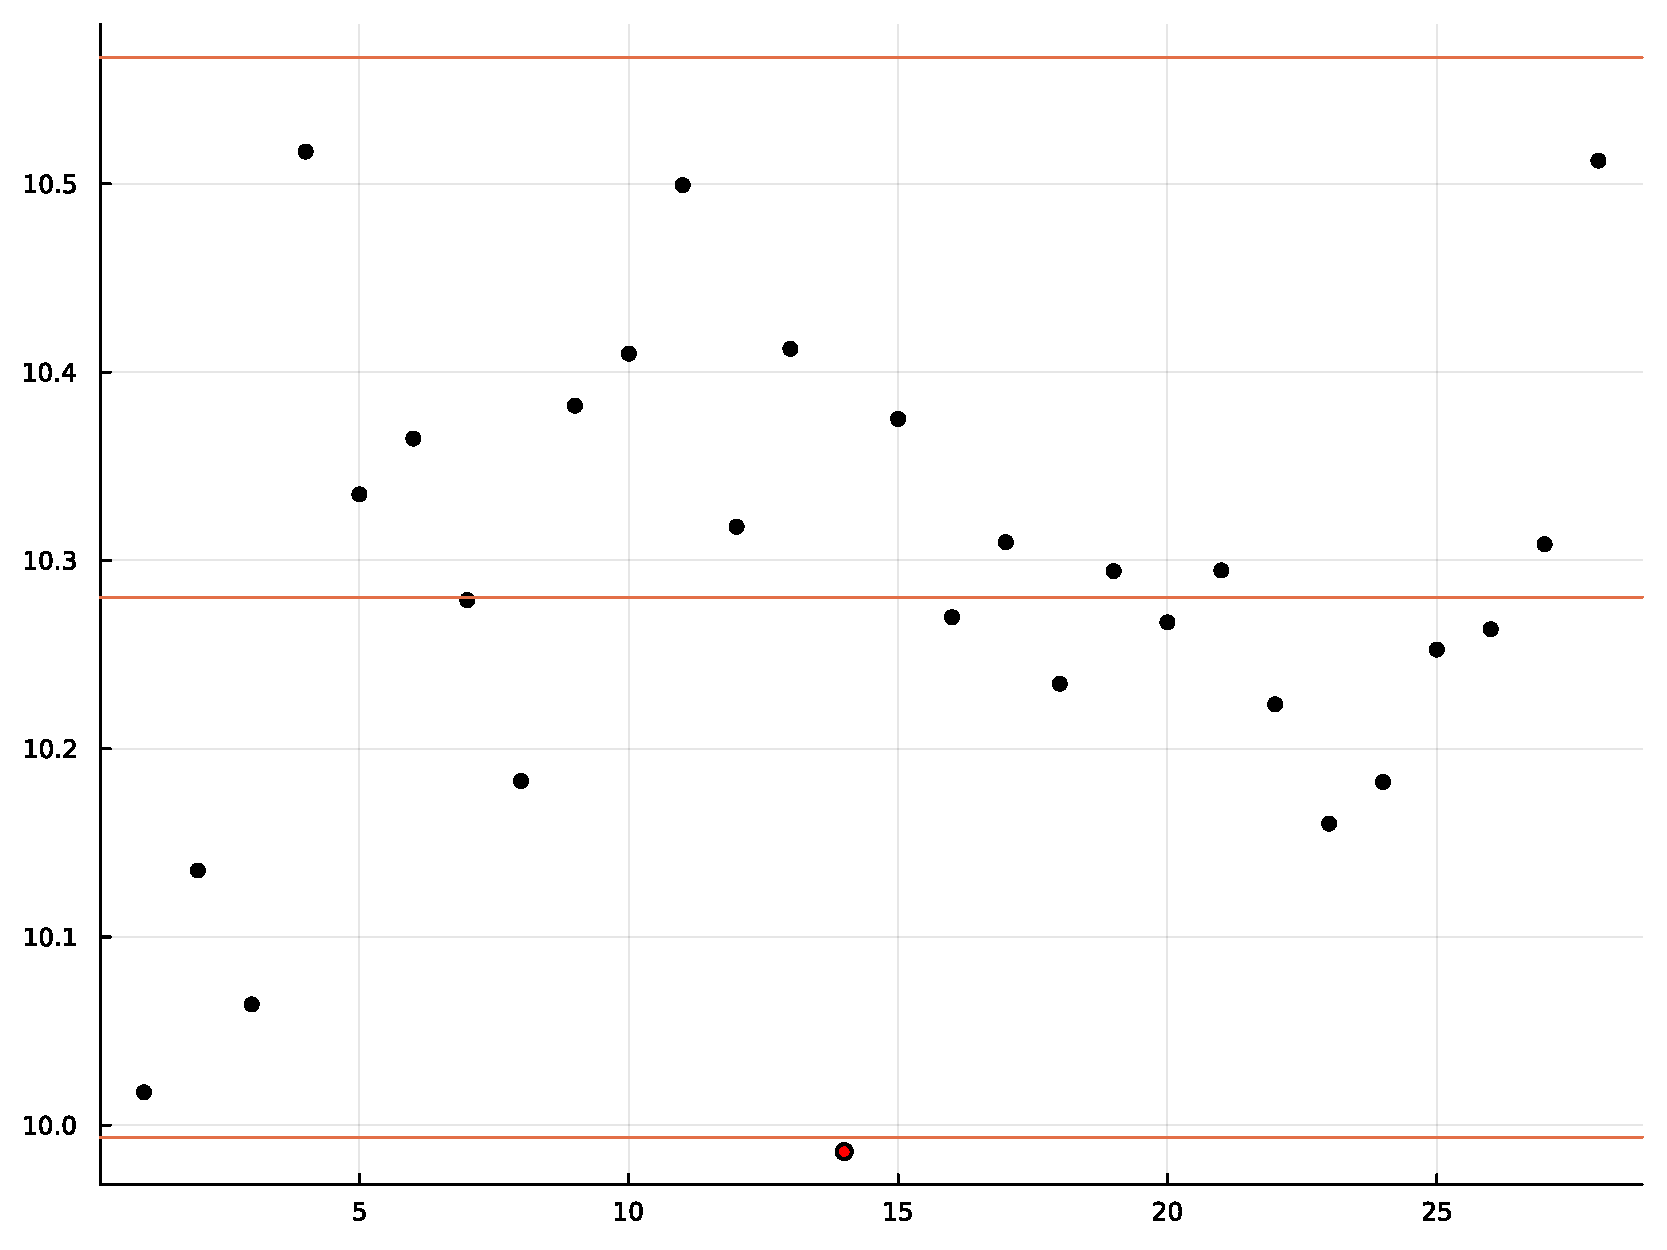
\includegraphics{trabalho1_files/figure-pdf/fig1-output-1.pdf}

}

\caption{Gráfico de controle da Média utilizando Amplitude}

\end{figure}

\begin{figure}

{\centering 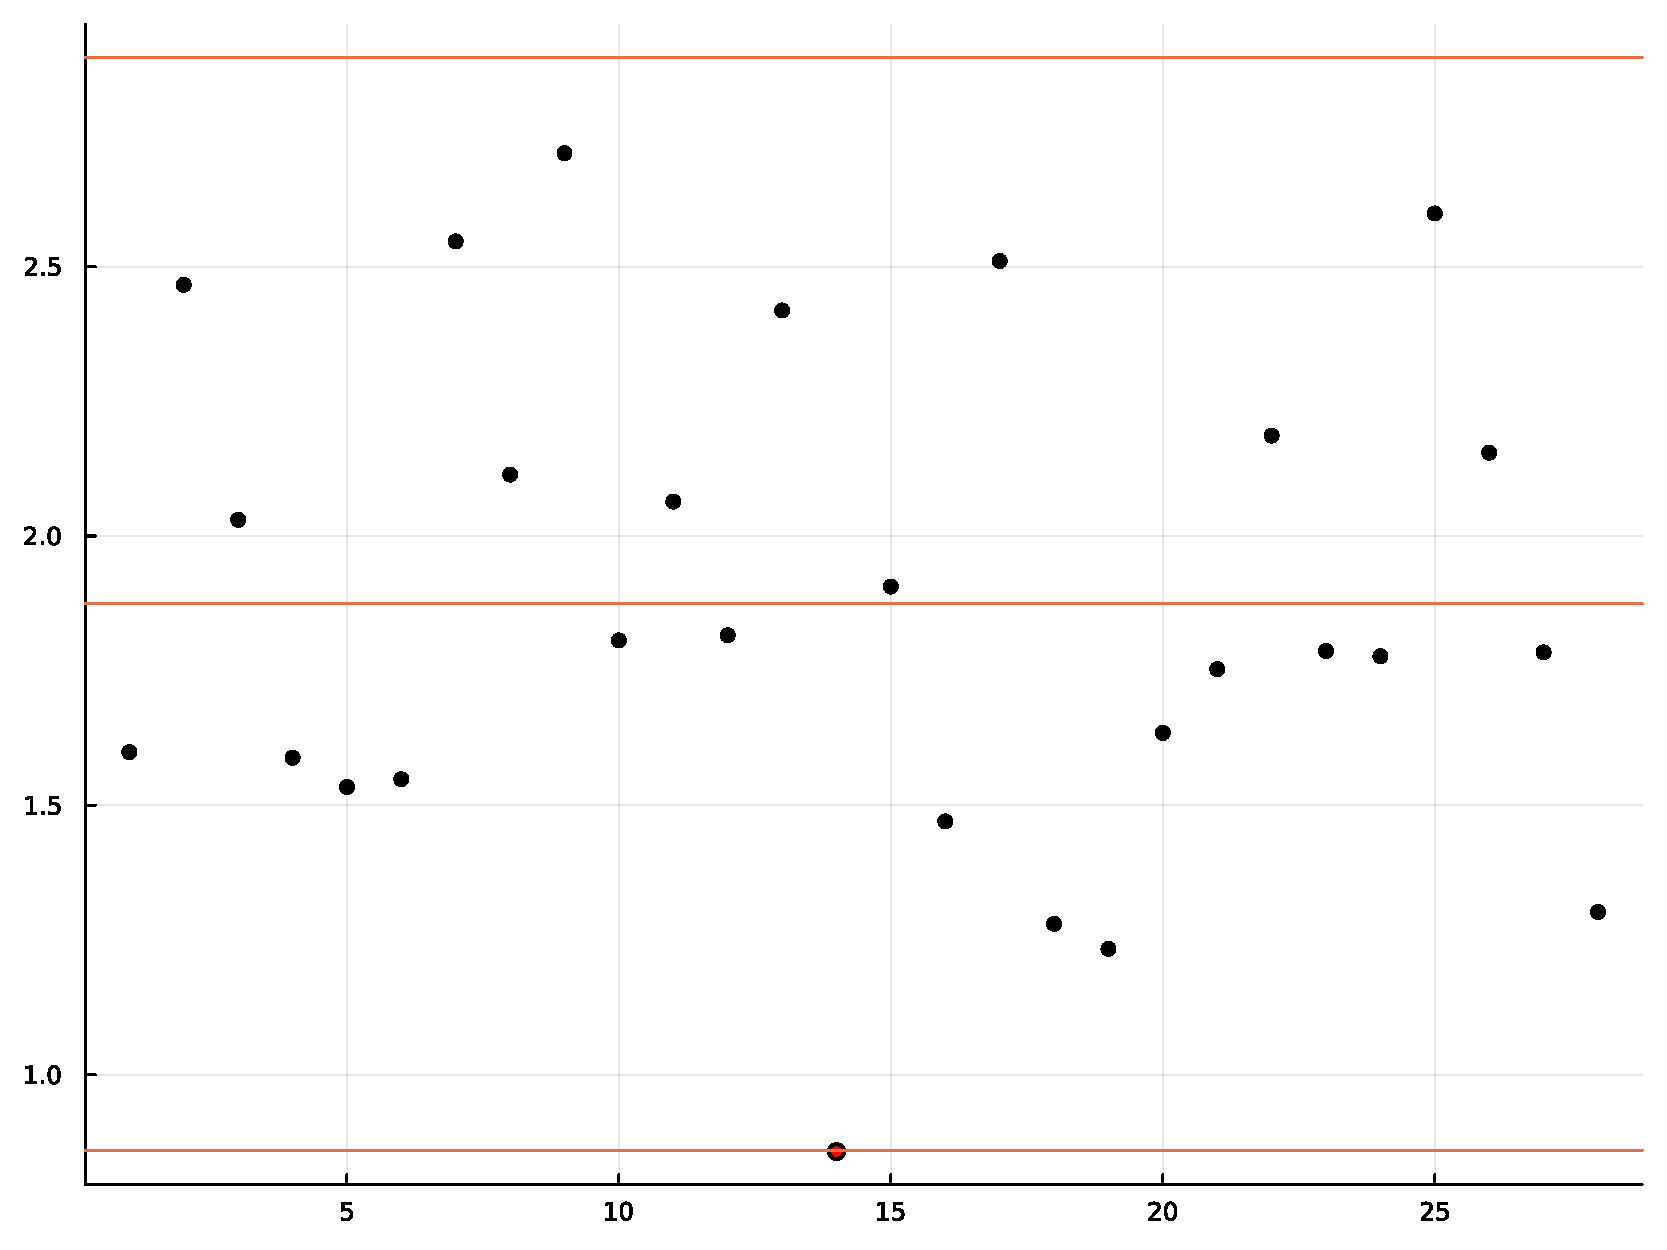
\includegraphics{trabalho1_files/figure-pdf/fig2-output-1.pdf}

}

\caption{Gráfico de controle o desvio padrão utilizando Amplitude}

\end{figure}

As Figuras 3 e 4, utilizam como estimador do limite o desvio padrão,
nota-se que é menos rigoroso quanto a pontos fora de controle, onde a
amostra 14 não está mais nessa condição. Na Figura 5, podemos afirmar
essa afirmação visualmente, onde o limite superior tem valores maiores e
o limite inferior tem valores menores quando são estimados pelo desvio
padrão.

\begin{figure}

{\centering 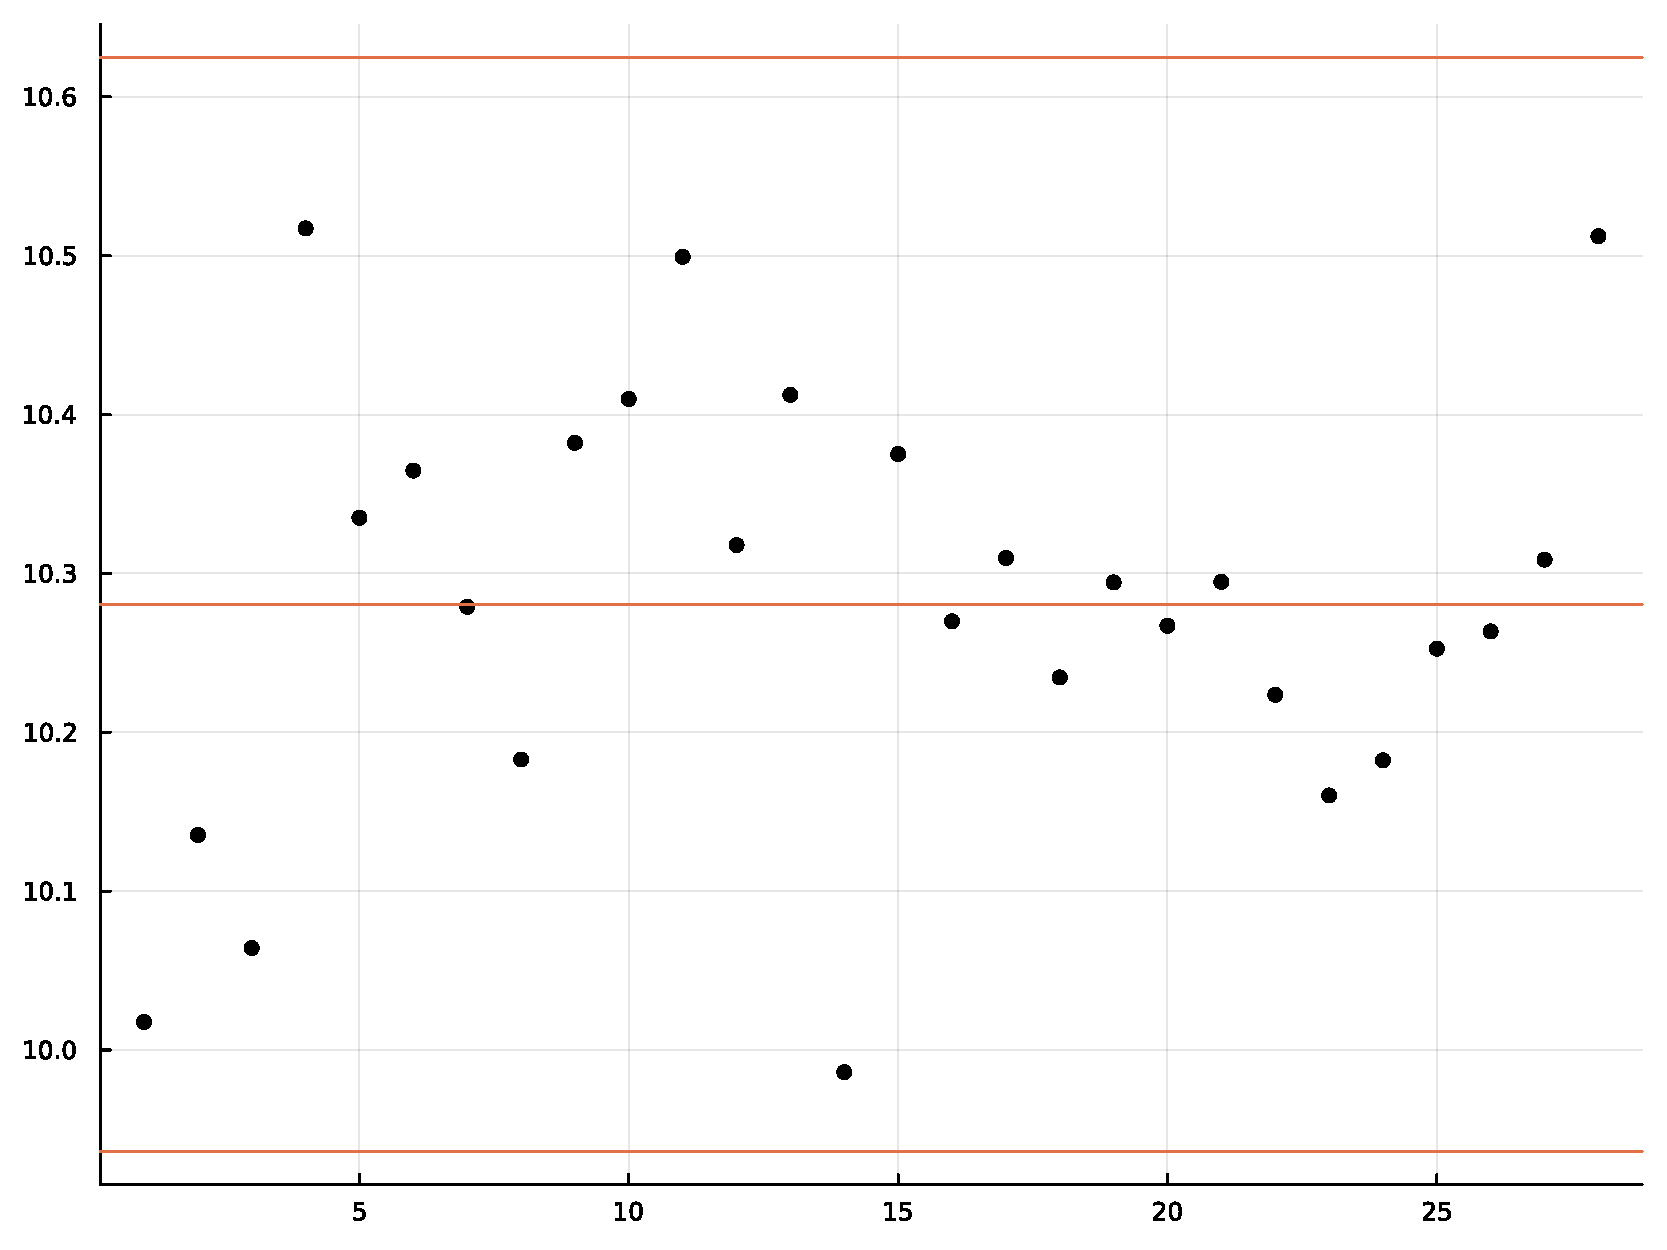
\includegraphics{trabalho1_files/figure-pdf/fig3-output-1.pdf}

}

\caption{Gráfico de controle da Média utilizando desvio padrão}

\end{figure}

\begin{figure}

{\centering 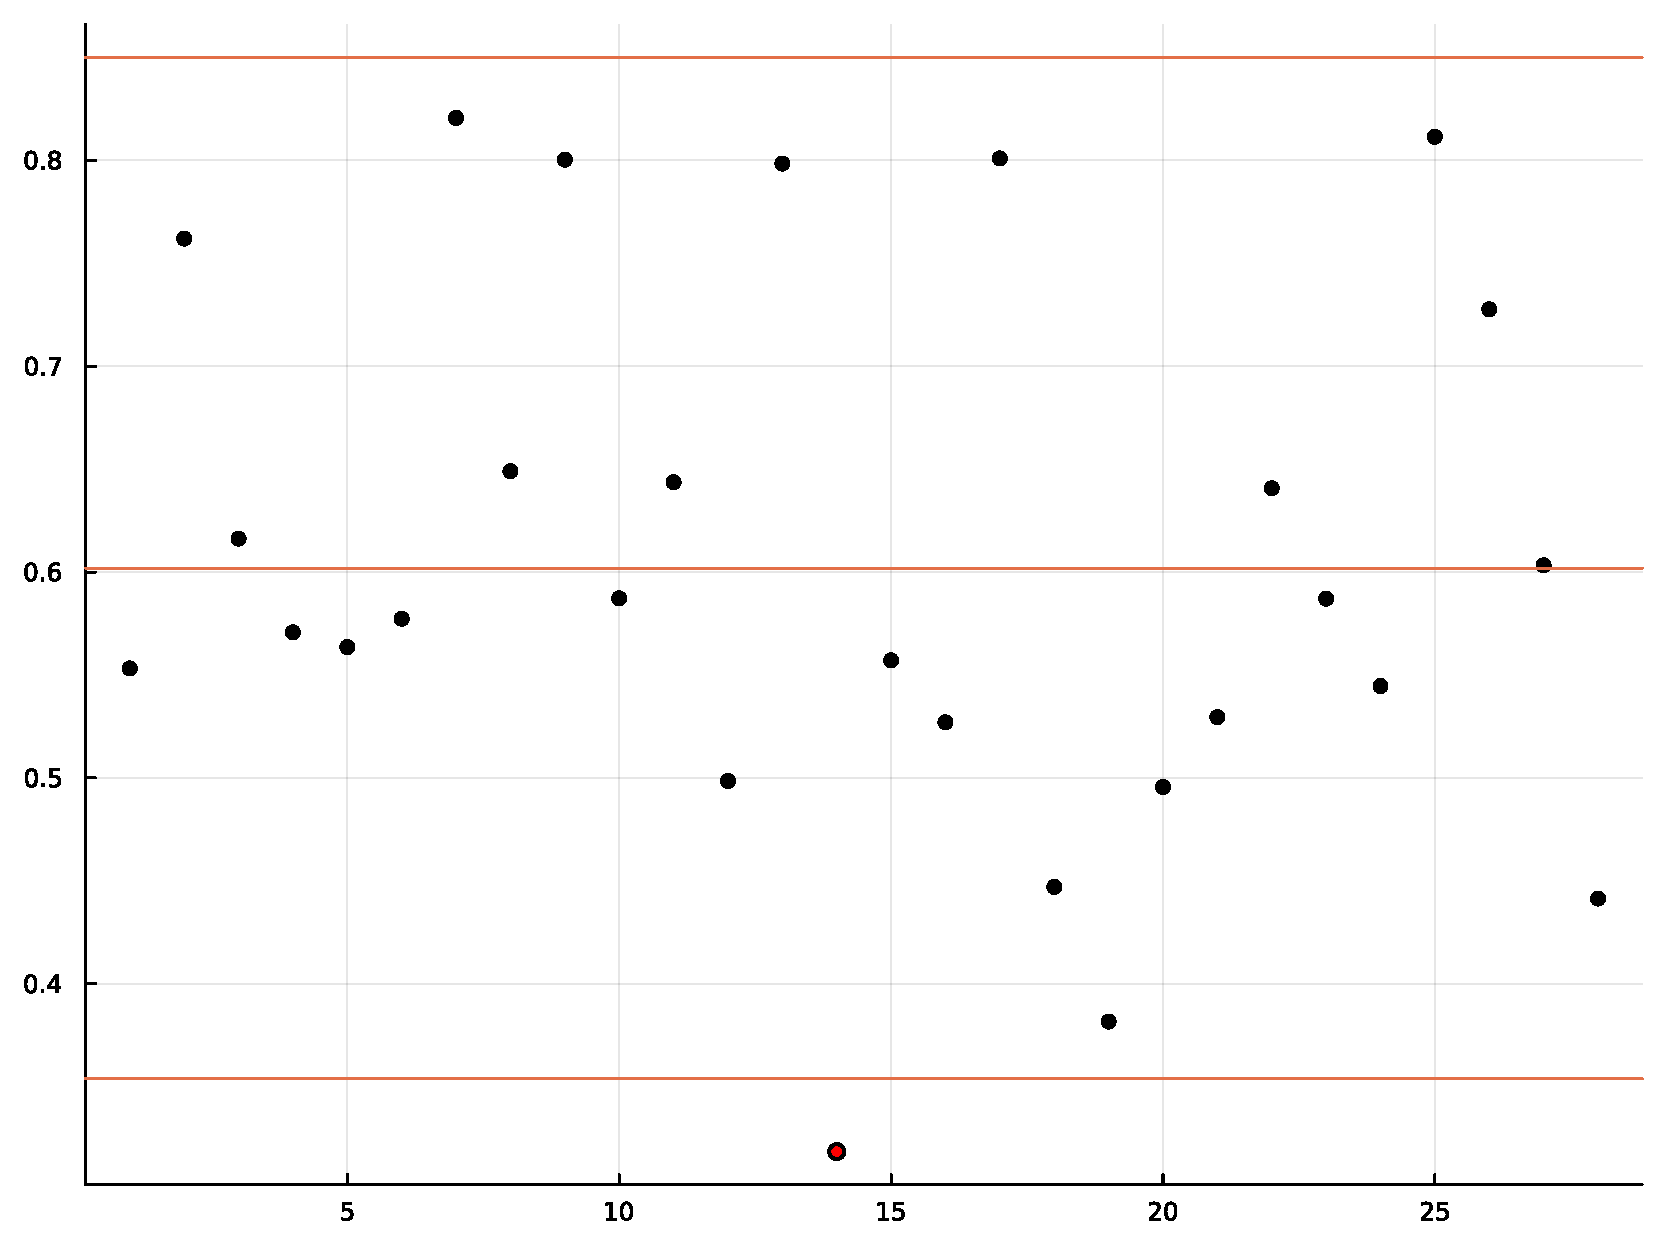
\includegraphics{trabalho1_files/figure-pdf/fig4-output-1.pdf}

}

\caption{Gráfico de controle o desvio padrão utilizando desvio padrão}

\end{figure}

\begin{figure}

{\centering 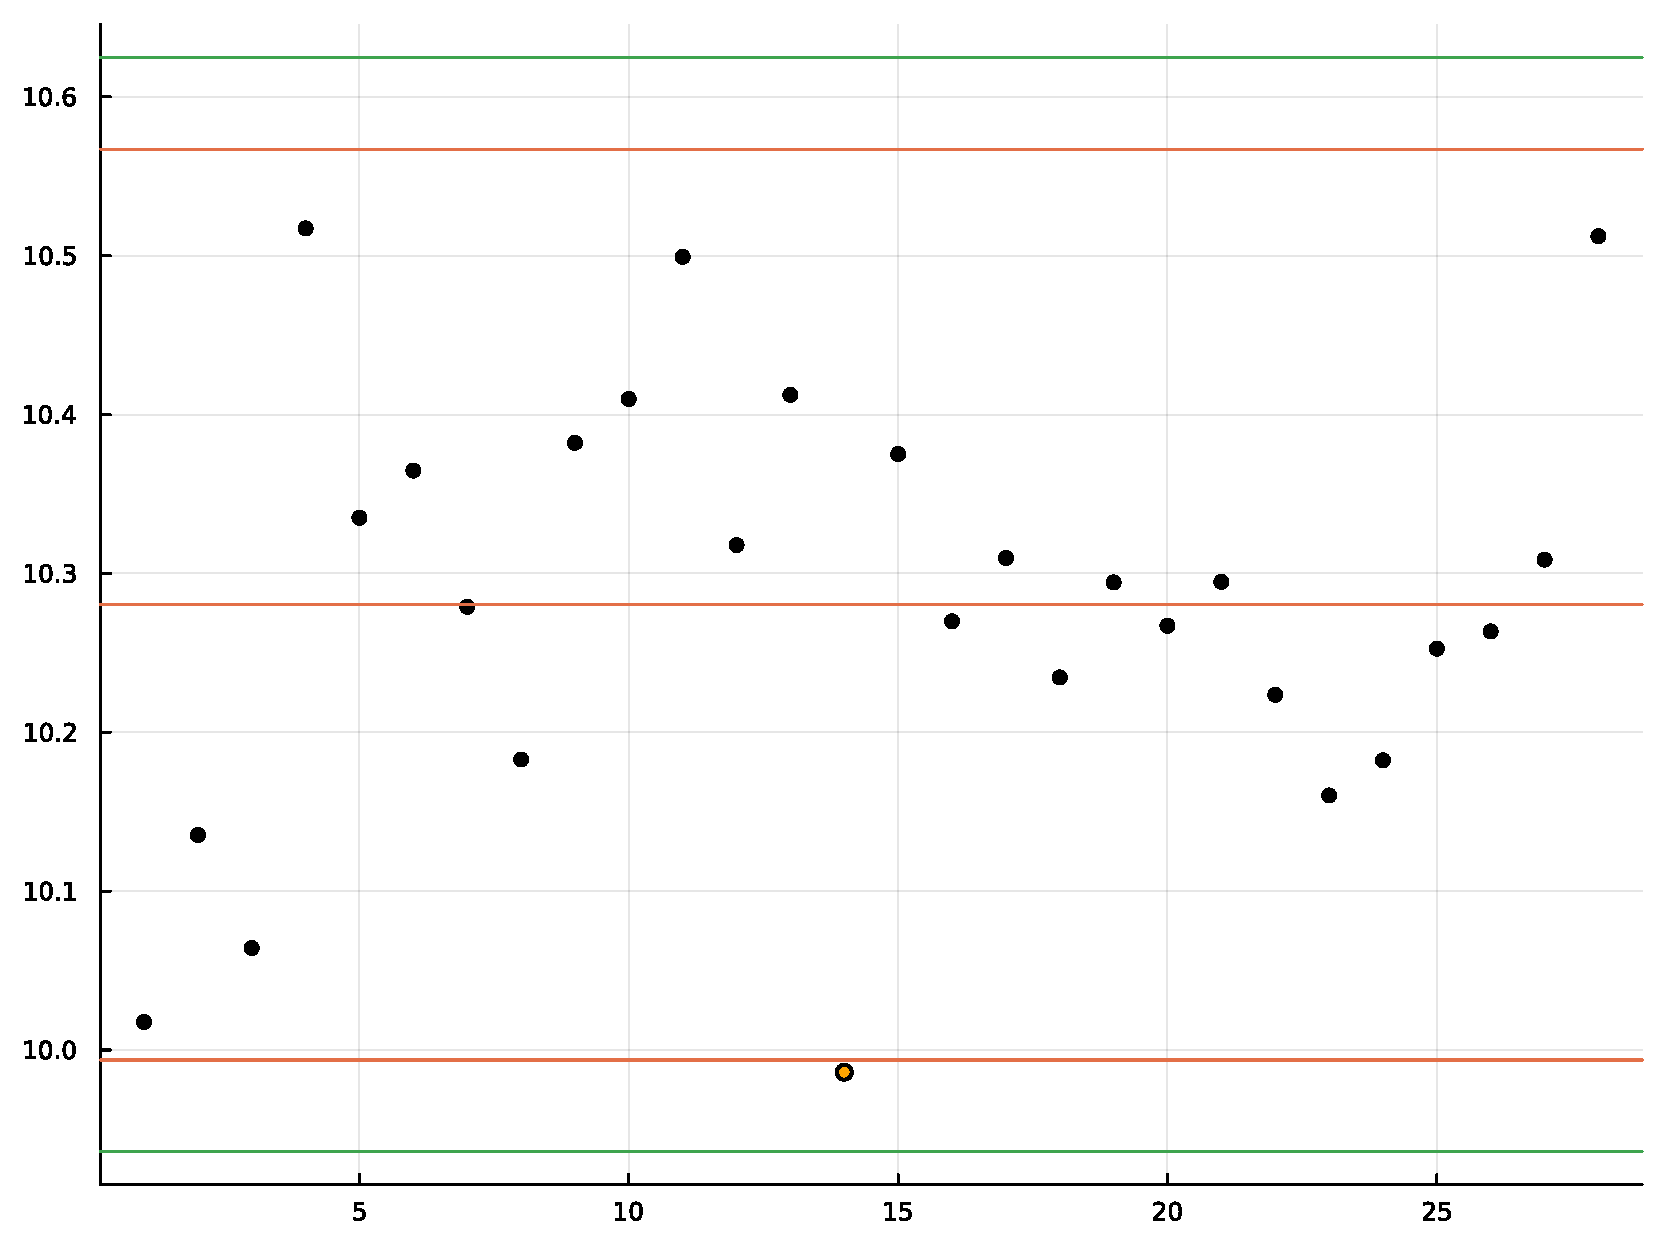
\includegraphics{trabalho1_files/figure-pdf/fig5-output-1.pdf}

}

\caption{Gráfico de controle da Média utilizando desvio padrão e
amplitude}

\end{figure}

\pagebreak

\subsection{Trabalho Aula}

No exemplo desenvolvido em aula temos um processo fora de controle, em
que podemos notar vários pontos acima ou abaixo dos limites construídos.
Assim, é possível dizer que a execução do trabalho ou cargo/função não
está com a qualidade necessária para um bom desenvolvimento do produto
ou outra atividade laboral.

\begin{verbatim}
2.345063708408997
\end{verbatim}

As Figuras 6 e 7, também utilizam como estimador do limite a amplitude,
onde é perceptível que quanto a média temos pontos fora de controle de
maneira exarcebada, sendo inclusive a maioria em relação aos pontos em
controle, no entanto, para o desvio padrão também temos alguns pontos
fora de controle, no entanto de maneira mais contida,tem-se 5 pontos
fora de controle, sendo dois deles novos em relação ao gráfico para
média, a amostra 5 e a amostra 13.

As Figuras 8 e 9, utilizam o desvio padrão para construção dos limites,
que como já notamos é menos rigoroso que a amplitude, assim nota-se uma
pequena queda de pontos fora de controle de 13 na Figura 6 para 11 na
Figura 8. No entanto, para o desvio padrão podemos notar que ocorre o
efeito contrário aumenta de 4 para 5 as amostras fora de controle,
quando o utilizamos a estimação dos limites pelo desvio padrão. Na
figura 10, fica de forma mais explícita a diferença entre os limites.

\begin{figure}

{\centering 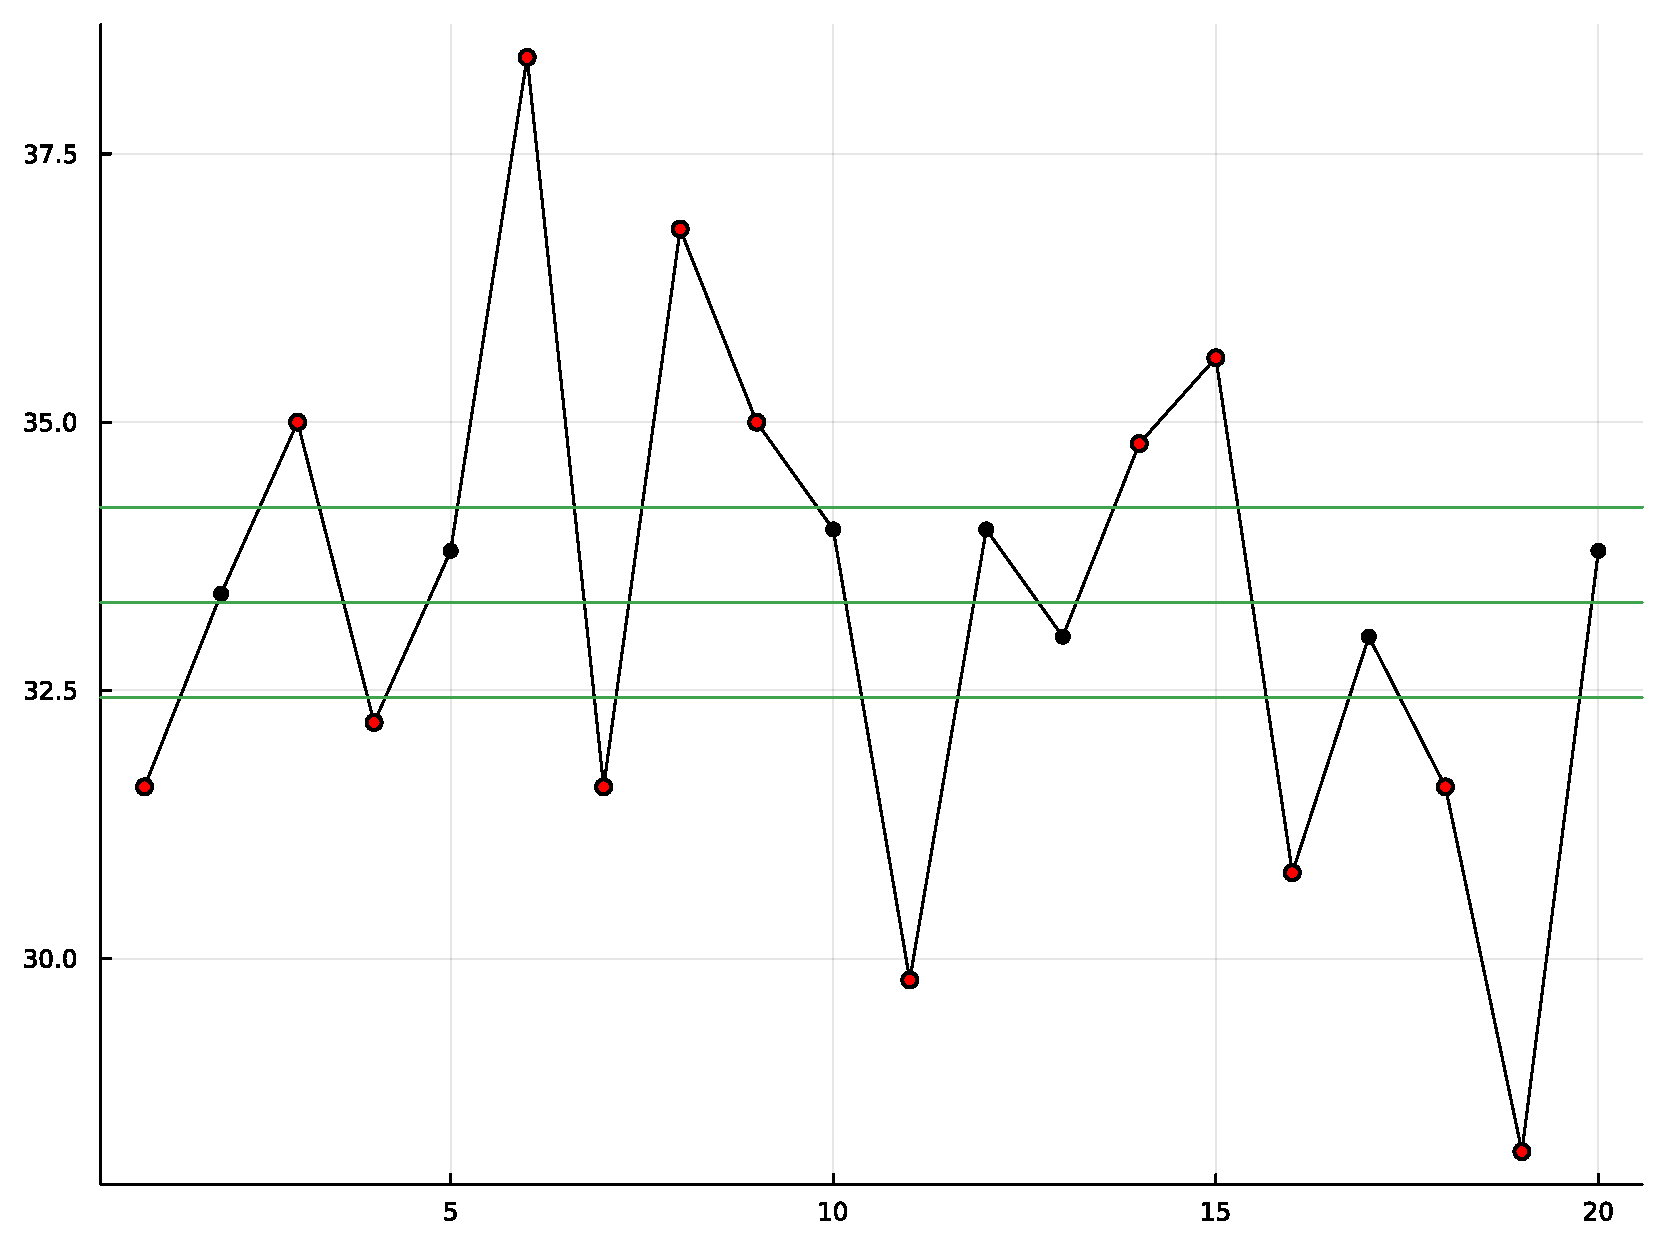
\includegraphics{trabalho1_files/figure-pdf/fig6-output-1.pdf}

}

\caption{Gráfico de controle da Média utilizando Amplitude - aula}

\end{figure}

\begin{figure}

{\centering 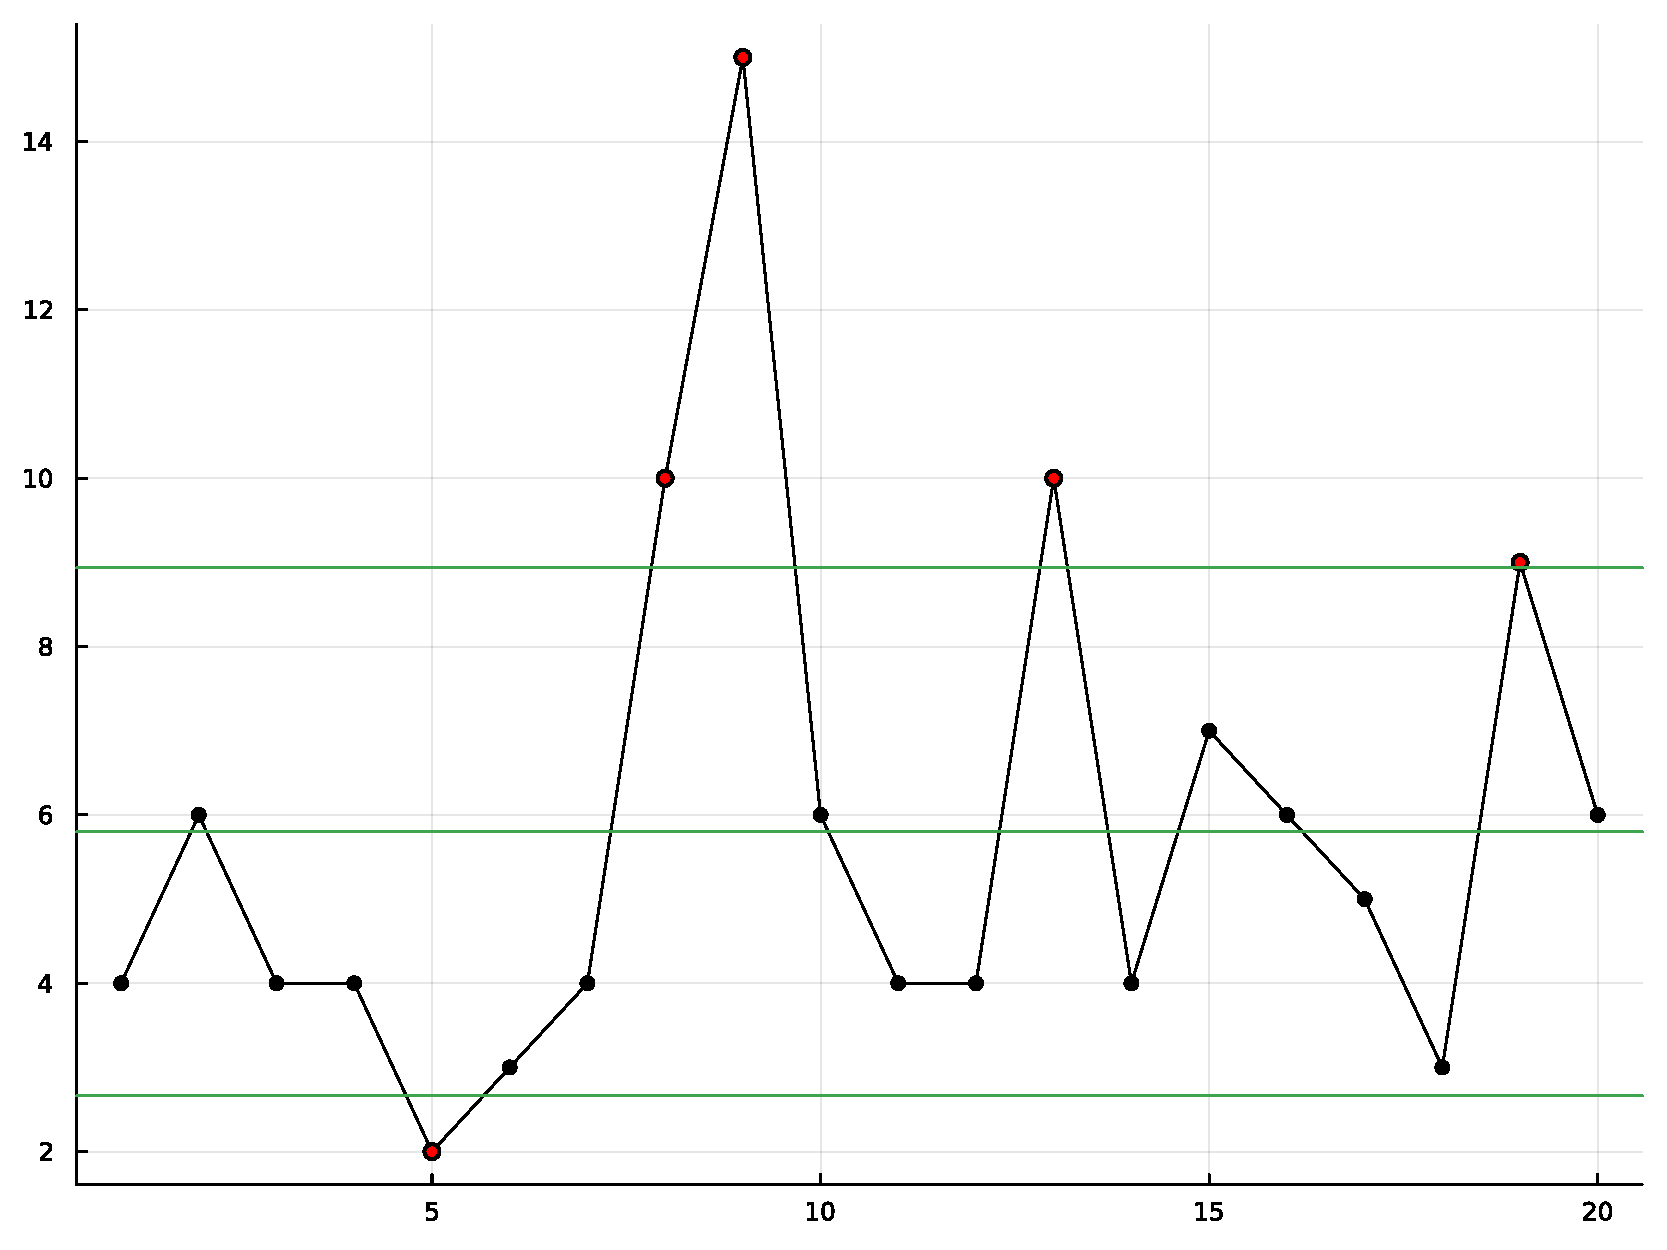
\includegraphics{trabalho1_files/figure-pdf/fig7-output-1.pdf}

}

\caption{Gráfico de controle o desvio padrão utilizando Amplitude -
aula}

\end{figure}

\begin{figure}

{\centering 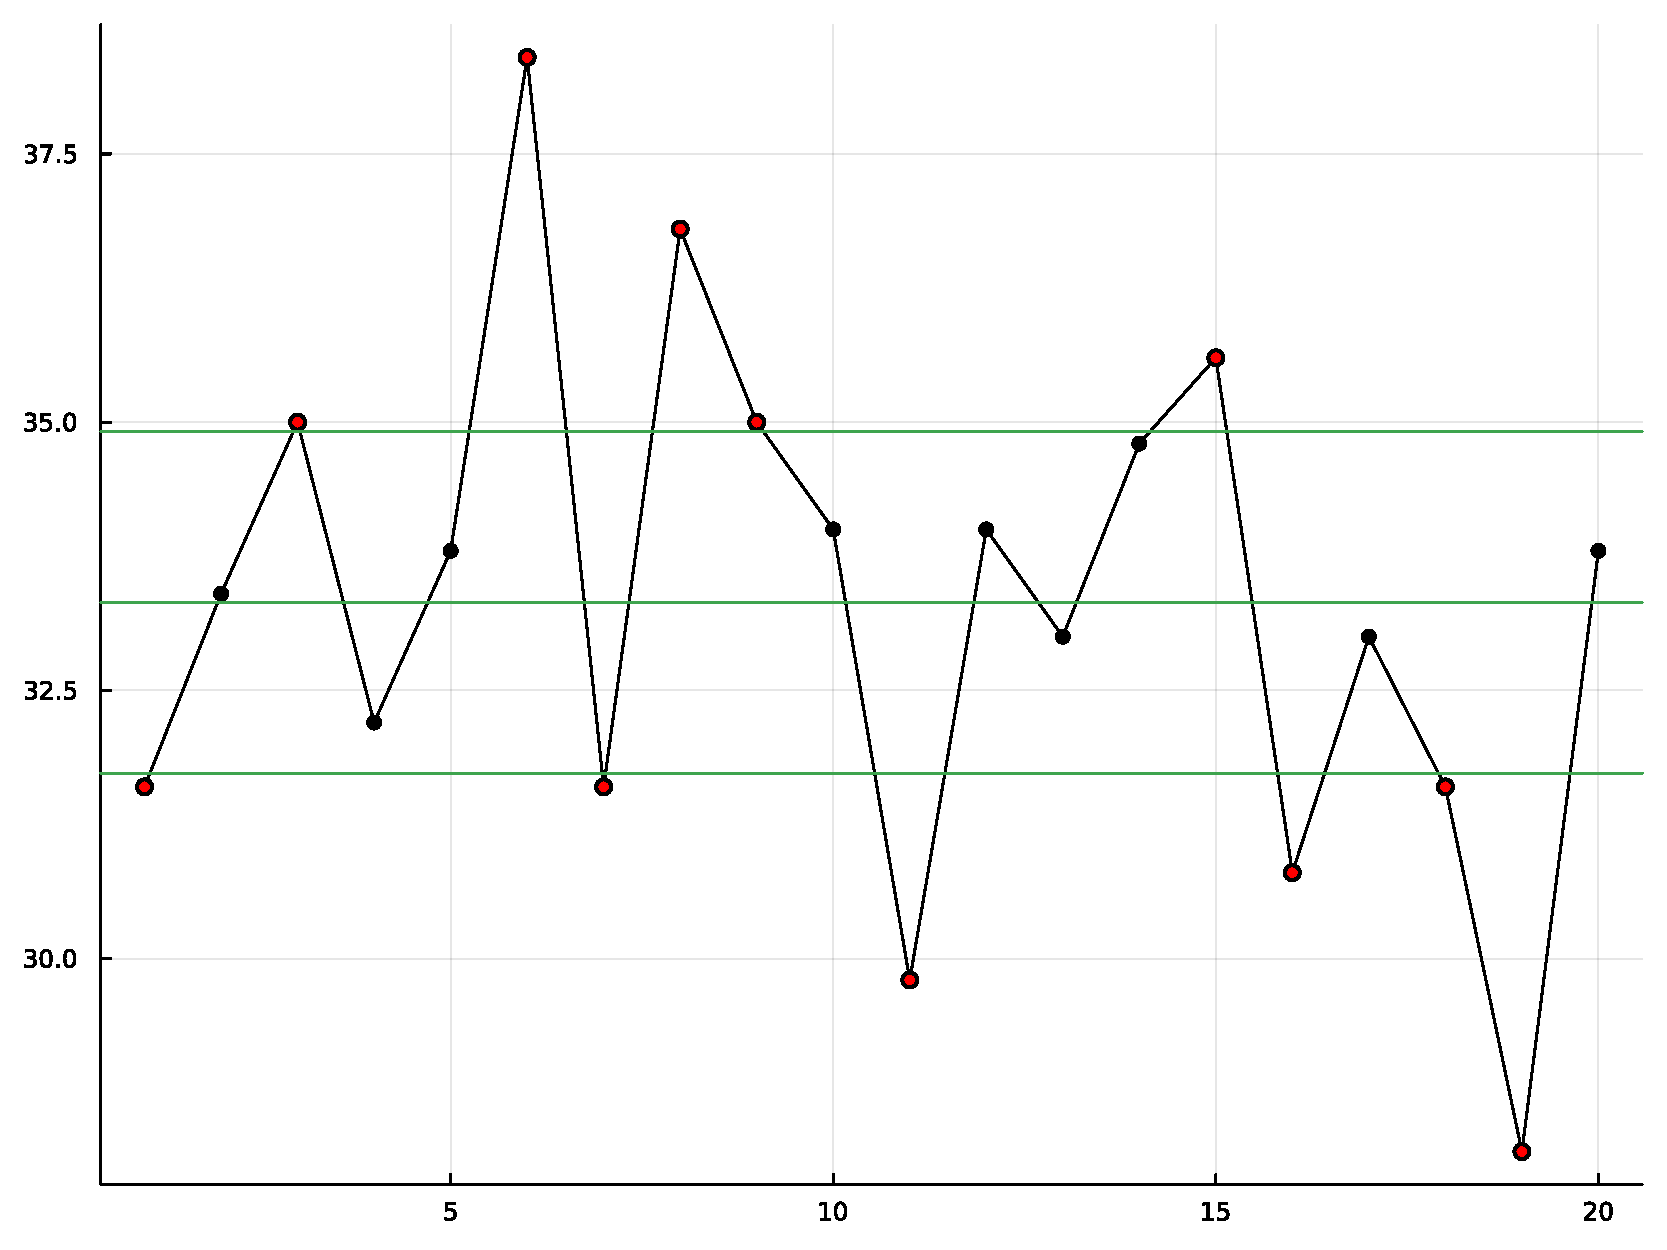
\includegraphics{trabalho1_files/figure-pdf/fig8-output-1.pdf}

}

\caption{Gráfico de controle da Média utilizando desvio padrão - aula}

\end{figure}

\begin{figure}

{\centering 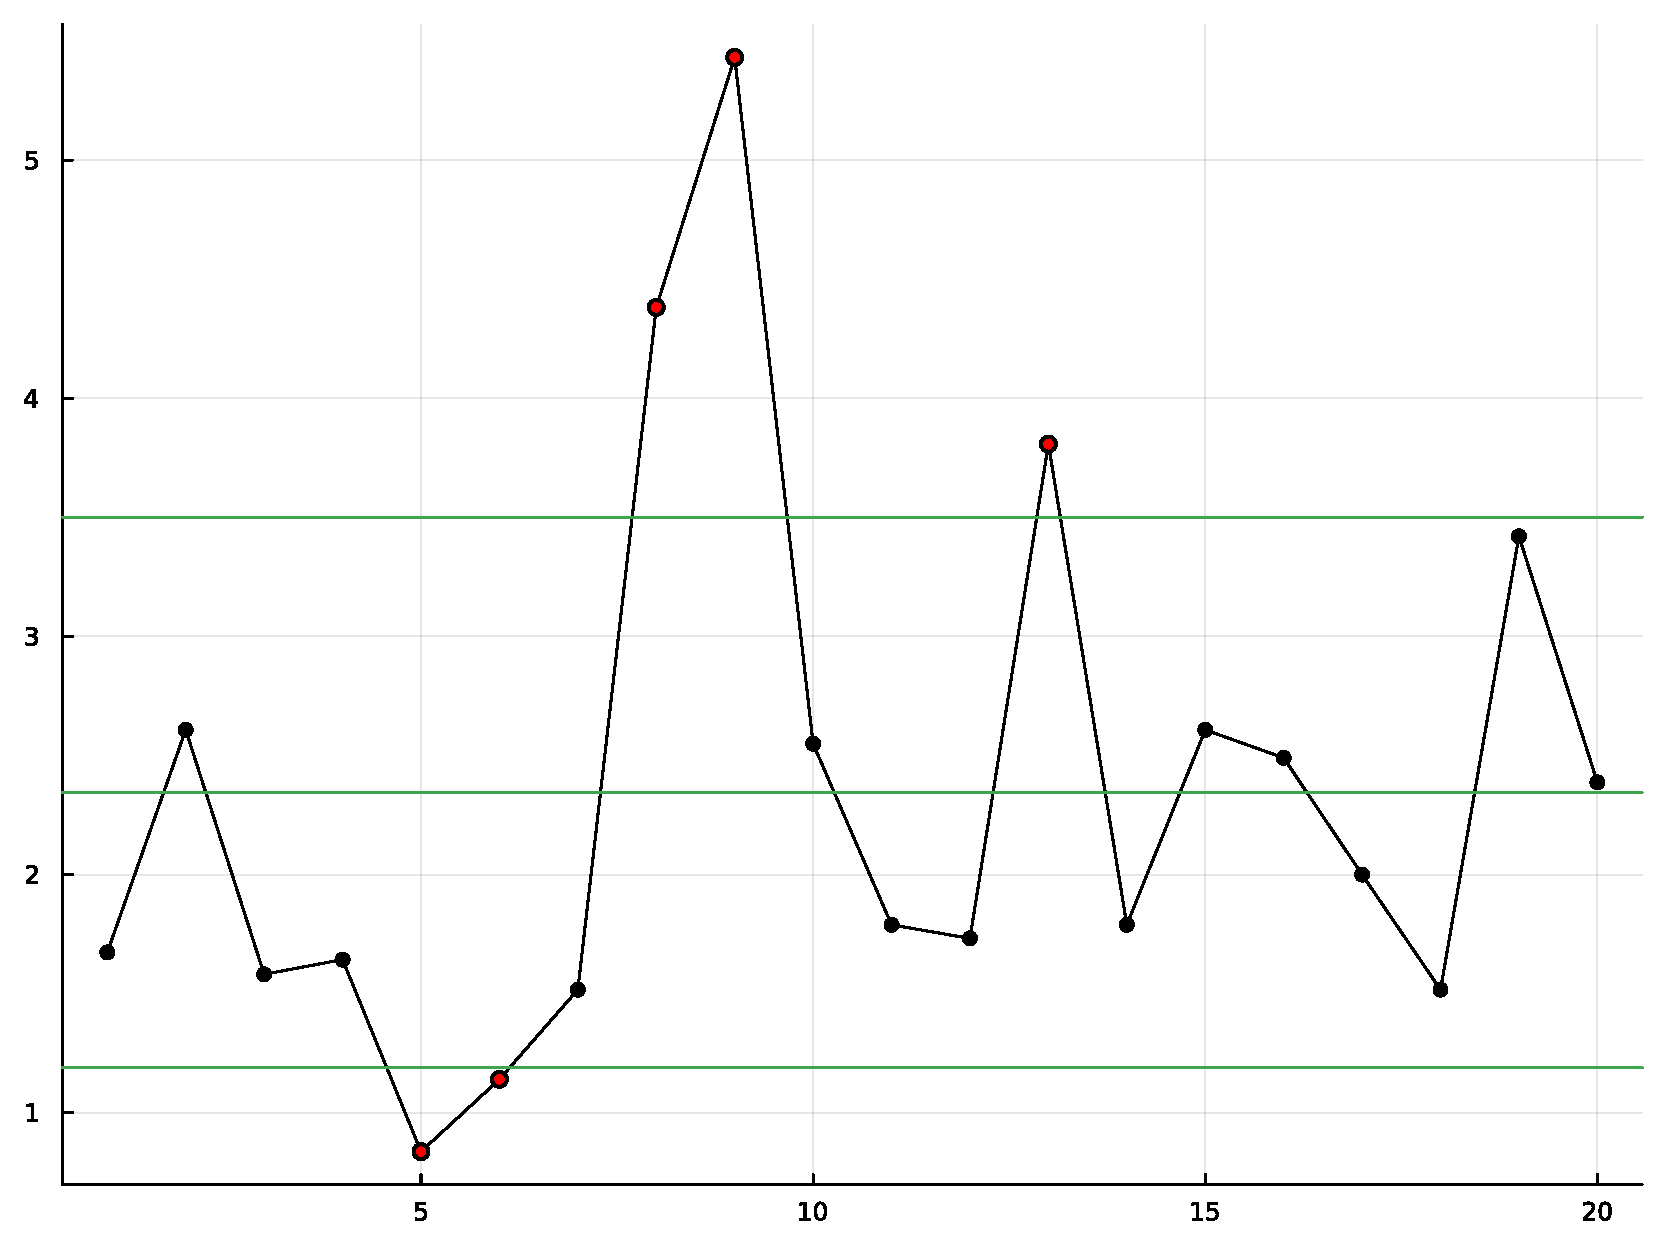
\includegraphics{trabalho1_files/figure-pdf/fig9-output-1.pdf}

}

\caption{Gráfico de controle o desvio padrão utilizando desvio padrão -
aula}

\end{figure}

\begin{figure}

{\centering 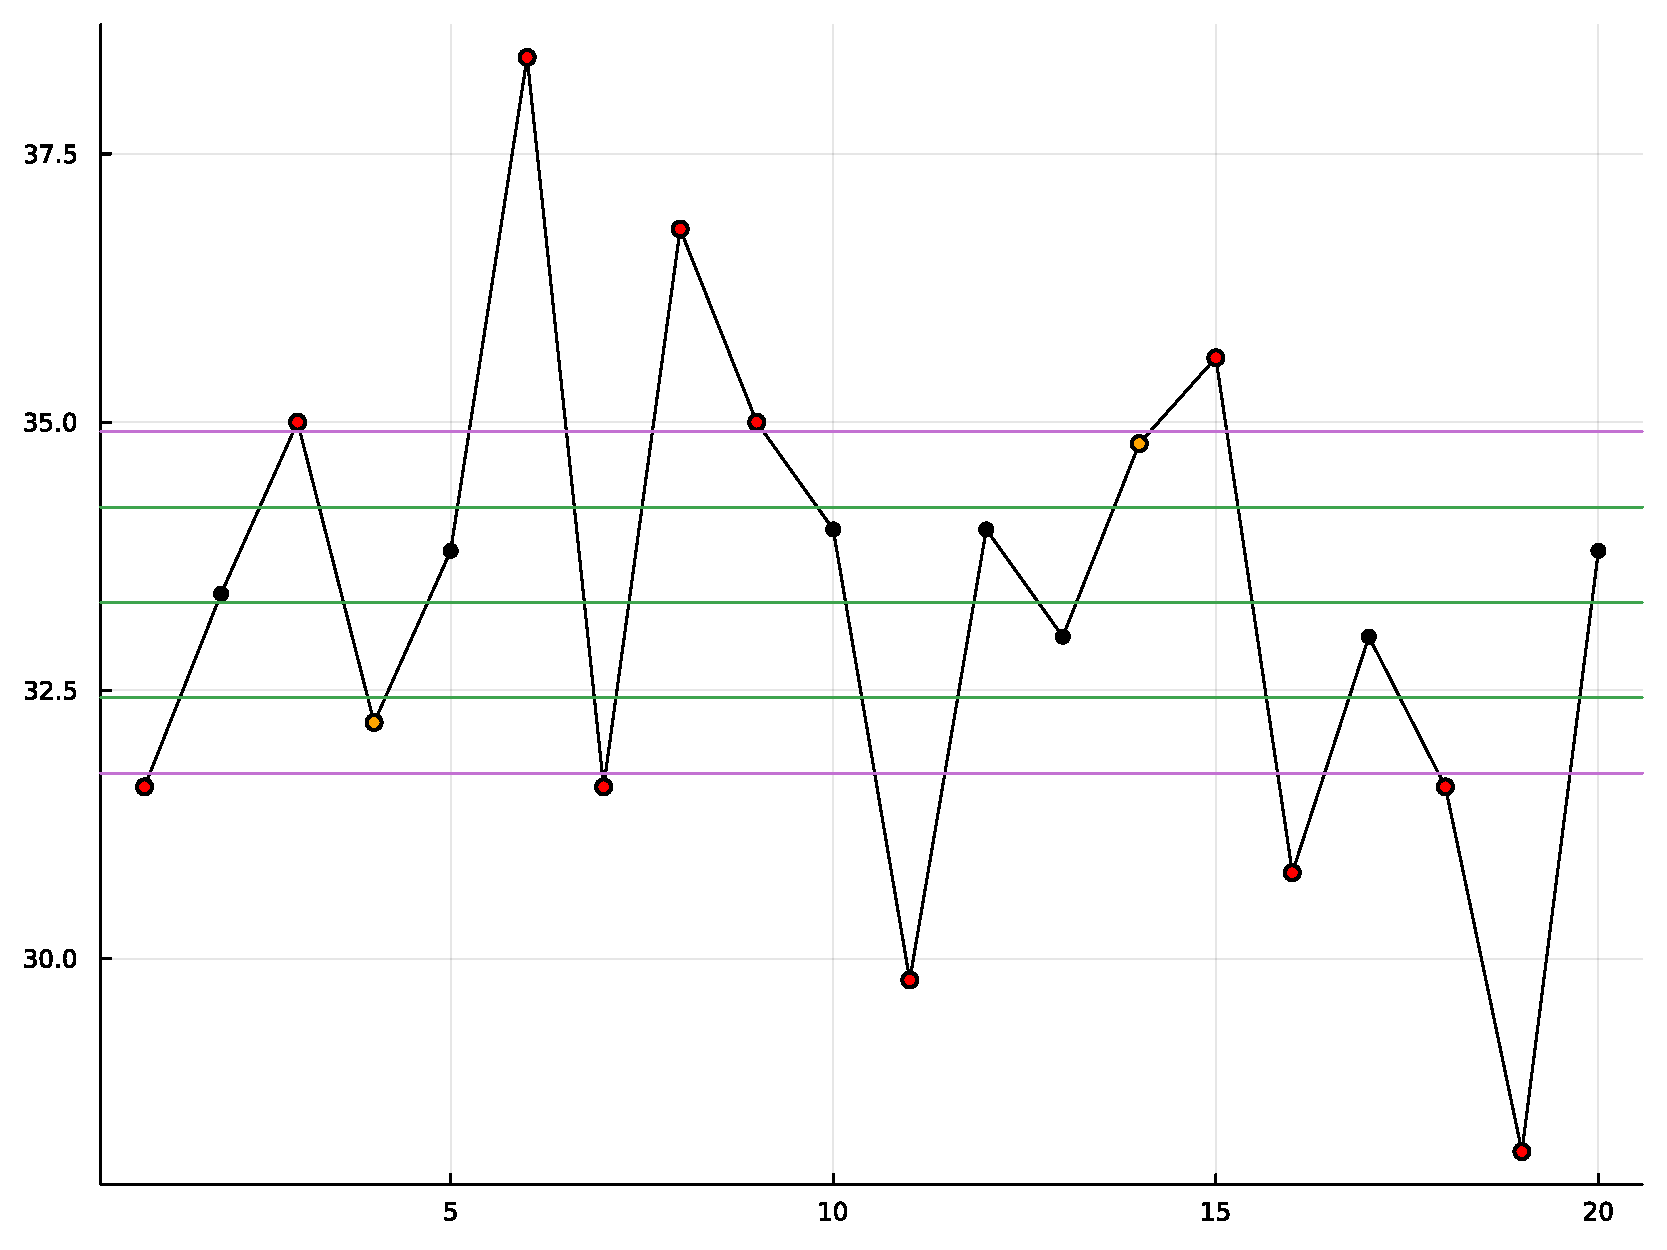
\includegraphics{trabalho1_files/figure-pdf/fig10-output-1.pdf}

}

\caption{Gráfico de controle da Média utilizando desvio padrão e
amplitude - aula}

\end{figure}

\begin{verbatim}
9.518556382978723
\end{verbatim}

\pagebreak

\section{Gráfico de controle para medidas individuais}

Para os gráficos de controle para medidas individuais, expostos na
Figura 11 e Figura 12, temos que todos os valores ficaram dentro dos
limites. Assim, podemos afirmar que tudo está ocorrendo com a qualidade
desejada, sem nenhum problema substancial a atividade que está sendo
construído, assim é possível afirmar que as atividades estão ocorrendo
sem nenhum padrão aleatório, logo dentro de controle.

\begin{figure}

{\centering 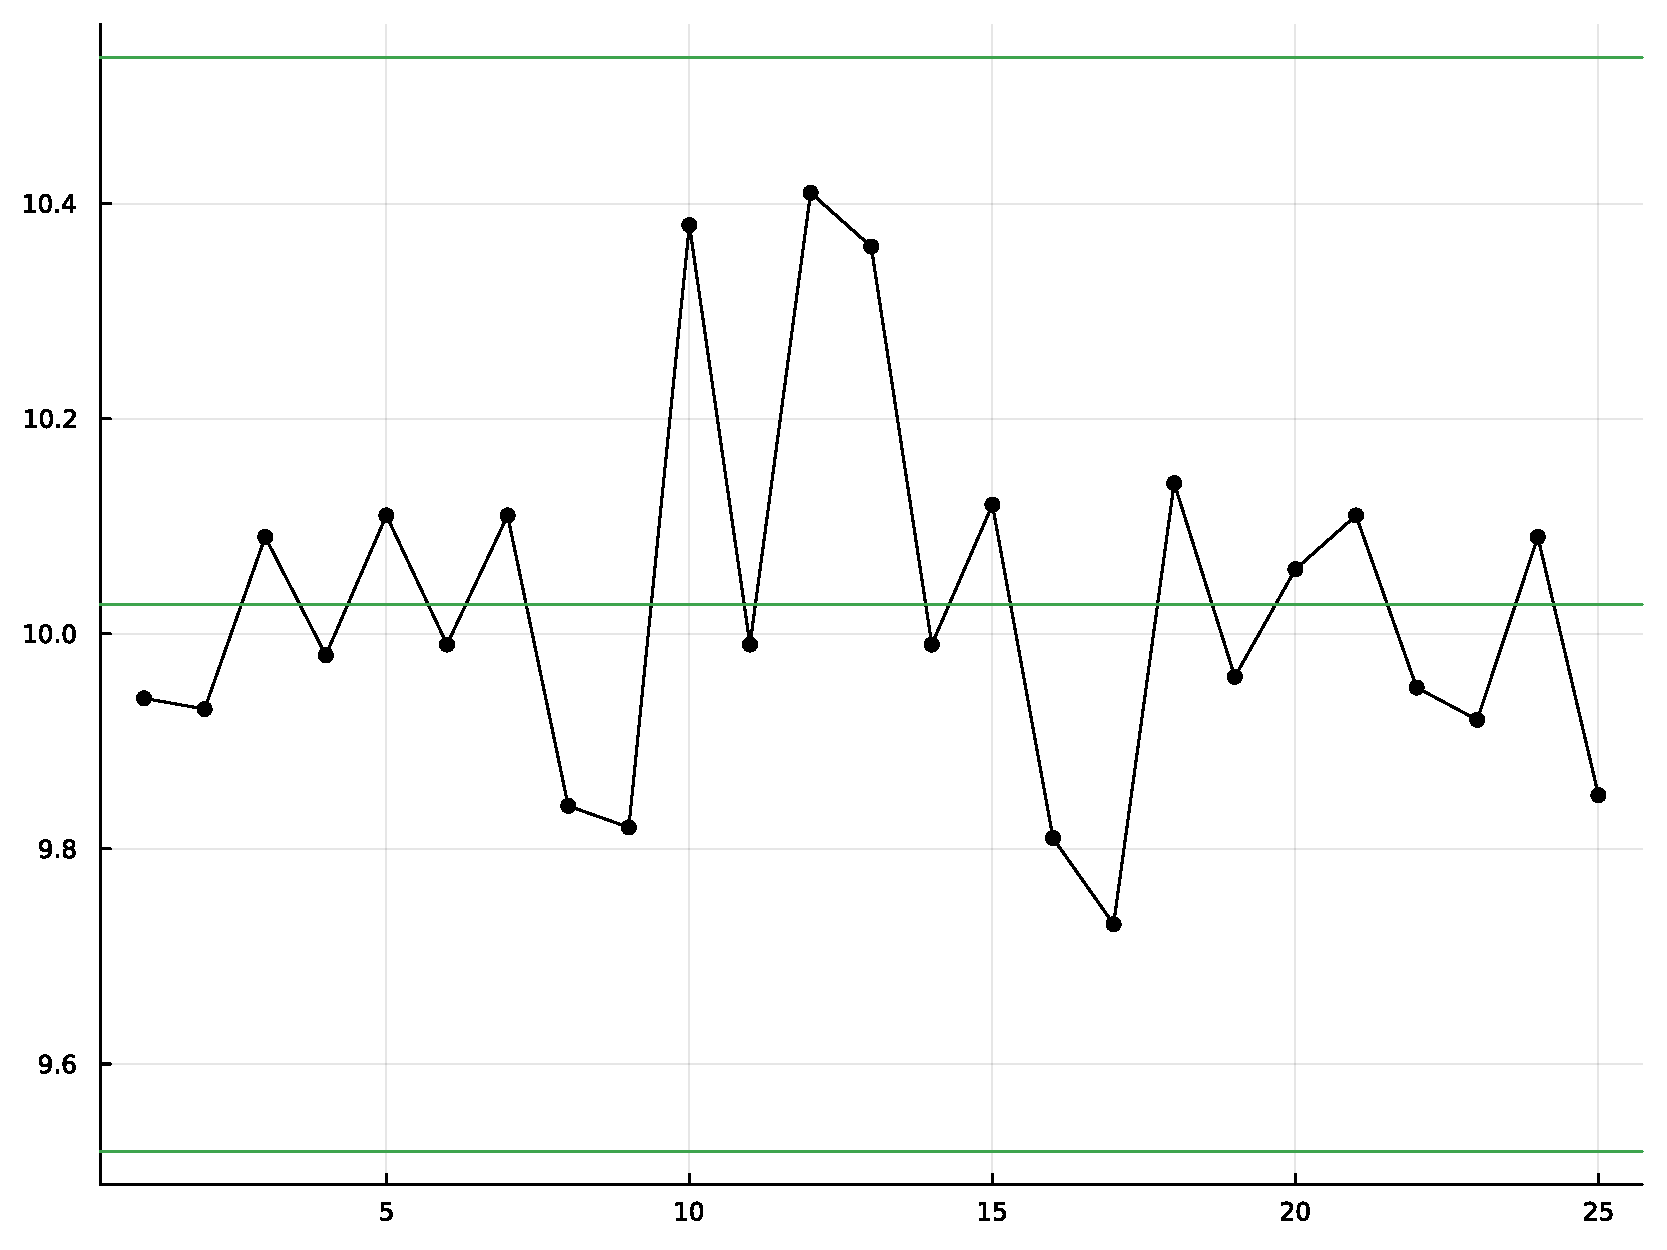
\includegraphics{trabalho1_files/figure-pdf/fig11-output-1.pdf}

}

\caption{Gráfico de controle para medidas individuais para o diâmetro}

\end{figure}

\begin{figure}

{\centering 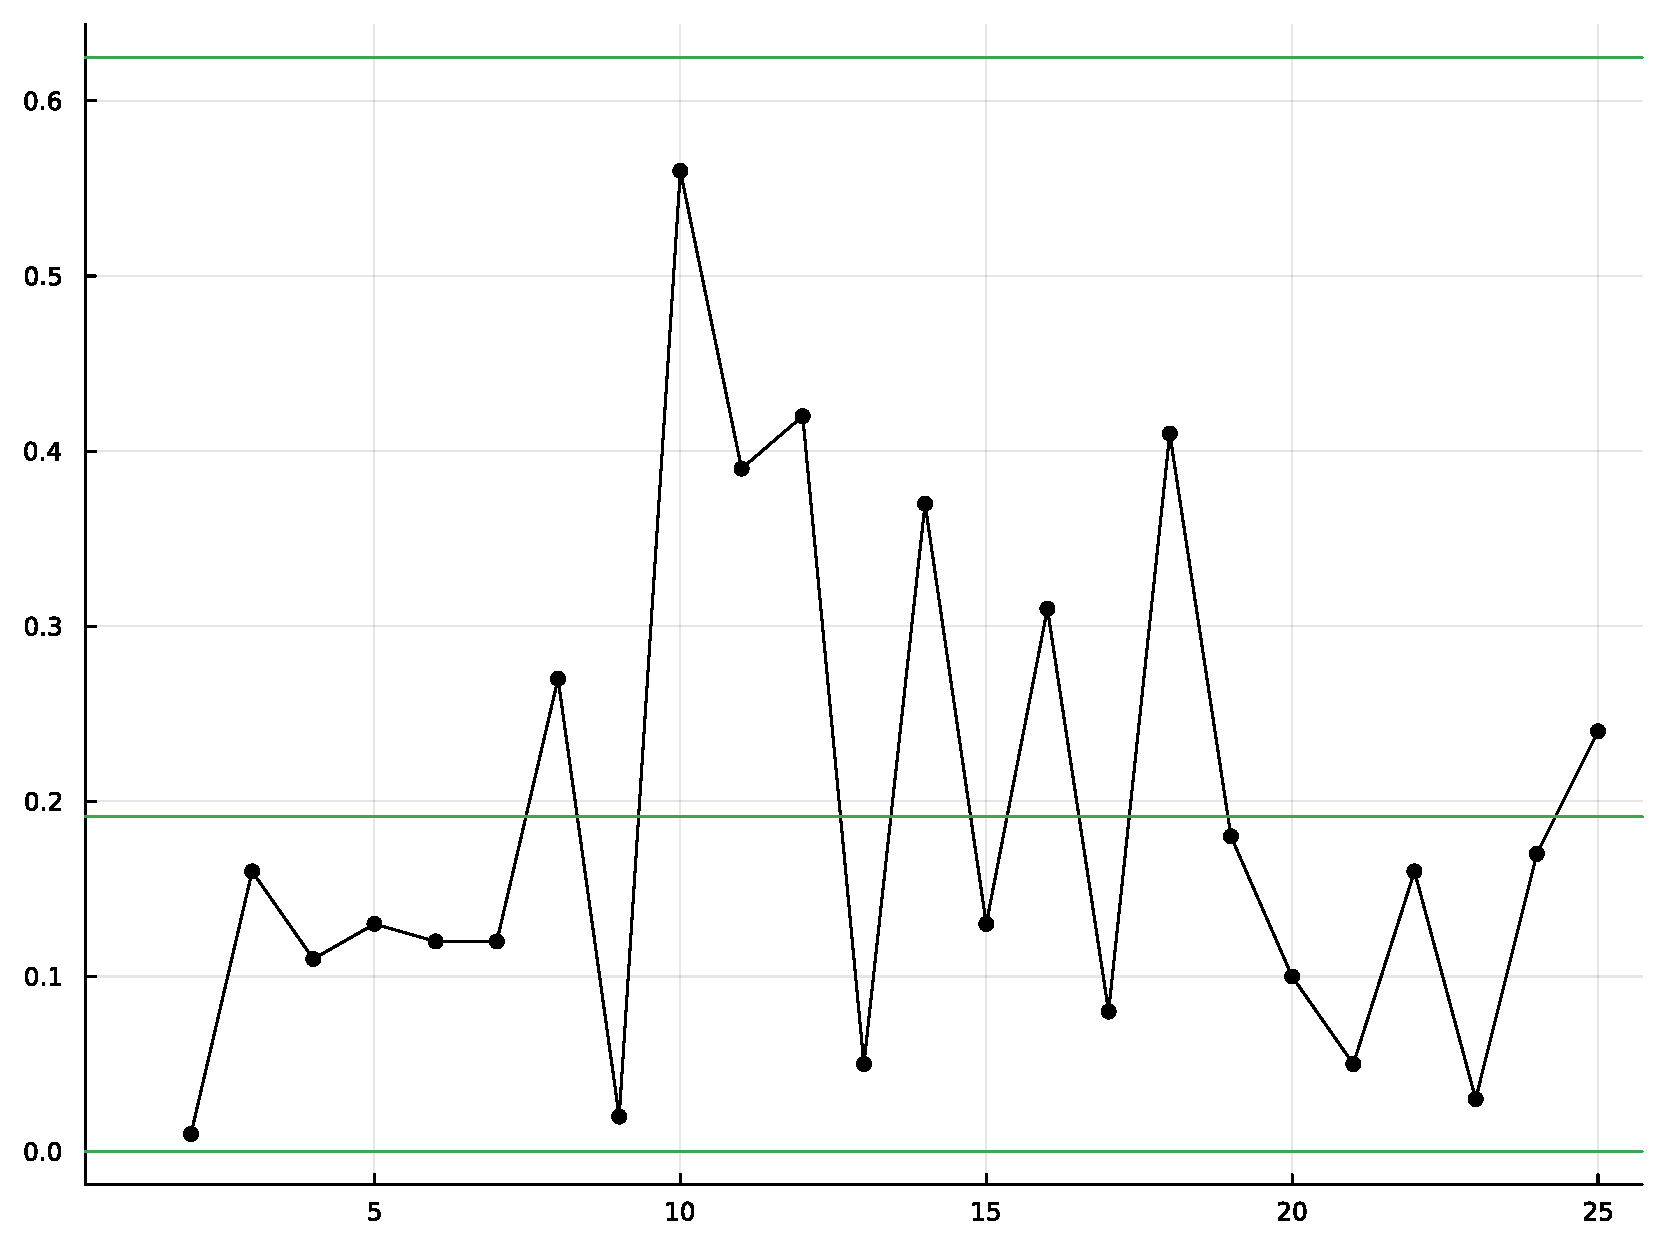
\includegraphics{trabalho1_files/figure-pdf/fig12-output-1.pdf}

}

\caption{Gráfico de controle para medidas individuais para a amplitude}

\end{figure}



\end{document}
